
\section{Tutorial}
\label{section:tutorial}
\setcounter{footnote}{0}

Here's a tutorial walk-through of some how to use \rscape. This should
suffice to get you started.

\subsection {Modes of \rscape}

\begin{tabular}{ll}
\multicolumn{2}{c}{\textbf{MSA input with annotated consensus secondary structure}} \\ 
 & \\ 
\textbf{R-scape}   & Reports all pairs which covariation scores have E-values smaller or equal to a target E-value.\\
\textbf{}          & Draws the given consensus structure annotated with the significantly covarying base pairs.\\
 & \\ 
\multicolumn{2}{c}{\textbf{MSA input without an annotated secondary structure}}  \\
 & \\ 
\textbf{R-scape}   & Reports all pairs which covariation scores have E-values smaller or equal to a target E-value.\\
\textbf{}          & Builds the best consensus structure that includes all significantly covarying pairs,\\
\textbf{}          & \hspace{5mm}\emph{the maximum-covariation consensus structure}.\\
\textbf{}          & Draws the \emph{maximum-covariation consensus structure} annotated with the significantly covarying base pairs.\\
 & \\ 
\end{tabular} \\
\\

In the Tutorial section, I'll show examples of running each \rscape,
using examples in the \ccode{tutorial/} subdirectory of the
distribution.


\subsection{Files used in the tutorial}

The subdirectory \prog{/tutorial} in the \rscape\ distribution contains the
files used in the tutorial. 

The tutorial provides several examples of RNA structural
alignments, all in Stockholm format:

\begin{sreitems}{\emprog{updated\_Arisong.sto}}
\item[\emprog{updated\_Arisong.sto}] Structural alignment of the ciliate
  Arisong RNA. This alignment is an updated
  version of the one published in~\citep{JungEddy11}.
\item[\emprog{ar14.sto}] Structural alignment of the $\alpha$-proteobacteria ncRNA ar14. This alignment is an updated version of the one
  published in~\citep{delVal12}.
\item[\emprog{RF00005.sto}] Rfam v12.0~\citep{Nawrocki15} seed alignment of tRNA. 
\item[\emprog{RF00001.sto}] Rfam v12.0 seed alignment of YRNA. 
\item[\emprog{RF00001-noss.sto}] Rfam v12.0 seed alignment of 5S rRNA, after removing the consensus secondary structure. 
\end{sreitems}


\subsection{Running \rscape\, on one alignment file}
To run \rscape\ with default parameters on alignment file
\prog{tutorial/updated\_Arisong.sto} use:\\

\user{bin/R-scape tutorial/updated\_Arisong.sto}\\

\noindent
Default parameters are:

\begin{sreitems}{\emprog{Pairwise percent identity:}}
\item[\emprog{Target E-value:}]default is 0.05. \rscape\, reports
  pairs which covariation score has E-value smaller or equal to the
  target value.  The target E-value can be changed with option
  \emprog{-E <x>}, $x >= 0$.

\item[\emprog{Pairwise percent identity:}]Sequences with more than
  97\% similarity to each other are removed.  Pairwise \% identity is
  defined as the ratio of identical positions divided by the minimum
  length of the two sequences. The maximum pairwise percentage
  identity in the alignment can be changed with option \emprog{-I
    <x>}, $0<x<=1$.

\item[\emprog{Gaps in columns}]Columns with more than 50\% gaps are
  removed. The gap threshold for removing columns can be modified
  using option \emprog{--gapthresh <x>} , $0<x<=1$.

\item[\emprog{Covariation statistic}]The default covariation statistic
  is the product-average corrected G-Test (equivalent to option
  \emprog{--GTp}).

\item[\emprog{Covariation Class}]\rscape\ uses the 16 component
  covariation statistic (C16), unless the number of sequences in the
  alignment is $\leq$ 8 or the length of the alignment is $\leq$ 50,
  in which case it uses the two-class covariation statistic (C2). A
  particular covariation class can be selected using either
  \emprog{--C16} or \emprog{--C2}.

  The threshold for the minimum number of sequences can be changed
  with option \prog{--nseqthresh <n>}.  The threshold for the minimun
  alignment length can be changed with option \prog{--alenthresh <n>}.

\item[\emprog{Null alignments:}]\rscape\ in order to estimate E-values
  produces 20 null alignments, unless the product of the number of
  sequences by the length of the alignment $<$ 10,000 in which case
  the number of null alignments is 50; or $<$ 1,000 in which case it
  is 100. The number of null alignments can be controlled with option
  \emprog{--nshuffle <n>}.
\end{sreitems}

A full list of the \rscape\ options is fund by using

\user{\rscape\ -h}

\subsection{Tabular output per input file}

The output file \prog{tutorial/updated\_Arisong.out} looks like this:

\begin{sreoutput}
more tutorial/updated_Arisong.out 
# MSA updated_Arisong_1 nseq 69 (95) alen 65 (150) avgid 65.16 (64.97) nbpairs 20 (20)
# GTp thresh Eval 0.050000 cov=41.310069 [-9.744726,89.076909] [2 | 9 20 11 | 45.000000 81.818182 58.064516] 
                93             104      43.65   6.01567e-06
*               94             110      43.17   4.29923e-05
*               96             108      65.95   0
*               98             106      89.08   0
...
\end{sreoutput}
The output is a list of significant pairs ordered by the first positions. \\

\begin{sreitems}{\emprog{Second and third columns}}
\item[\emprog{First column}] indicates whether the significant pair is
  part of the given structure (*), or not.  If the pair is not in the
  structure, we distinguish whether the pair is compatible with the
  given structure ($\sim$) o not, in which case it is a blank.

\item[\emprog{Second and third columns}] are the two positions of the
  pair. Positions are relative to the input alignment.

\item[\emprog{Forth column}] is the covariation score

\item[\emprog{Fifth column}] is the E-value. Significant positions
  have E-values $<< 1$.
\end{sreitems}

The output file \prog{tutorial/updated\_Arisong.out} includes two
comment lines per alignment in the file:

\begin{sreitems}{\emprog{Second comment line}}
\item[\emprog{First comment line}]describes properties of the
  alignment: number of sequence (nseq), alignment length (alen),
  average percentage identity (avgid), and number of base pairs
  (nbpairs).  Values in parenthesis correspond to the alignment as is
  given. Values not in parenthesis correspond to the analyzed
  alignment after the default filters have been applied.

\item[\emprog{Second comment line}]describes properties of the
  \rscape\ search: the covariation method (GTp), the E-value threshold
  (0.05), the score at that E-value (42.3), the range of scores for all
  pairs in the alignments (from -9.7 to 89.1), the number of covarying
  not base pairs (2), the number of covarying base pairs (9), the
  number of base pairs (20), and the total number of covarying pairs
  (11). Lastly we provide the sensitivity (SEN=45.0=9/20), positive
  predictive value (PPV=81.8=9/11), and F-measure (F=58.1 = 2 * SEN *
  PPV / (SEN+PPV)).
\end{sreitems}


\subsection{Outputs per alignment}
Two files are produced per alignment in the input file: \\

File \prog{tutorial/updated\_Arisong\_1.his} is a two column
histogram. The first column is the covariation score. The second
column is the observed (or expected according the
 
\begin{sreoutput}
more tutorial/updated_Arisong.his
46.926096       0.000485437
43.607534       0.000970874
35.438767       0.00145631
26.759452       0.00194175
25.993630       0.00242718
25.227808       0.00291262
24.461986       0.0038835
24.206712       0.00436893
23.951438       0.00485437
....
\end{sreoutput}


File \prog{tutorial/updated\_Arisong\_1.R2R.sto} is a Stockholm
formatted alignment that includes the input alignment annotated with
the consensus structure. This Stockholm file also includes the
additional annotation required to use the drawing program R2R.

It is possible that the resulting drawing will show parts of the
secondary structure occluded from each other (especially for long
RNAs).  Using this file, one can customize a different drawing of the
structure using the R2R documentation, provided in
\prog{lib/R2R/R2R-manual.pdf}.


\subsection{Graphical outputs per alignment}
Three plots are produced per alignment in the input file: 

\begin{figure}
  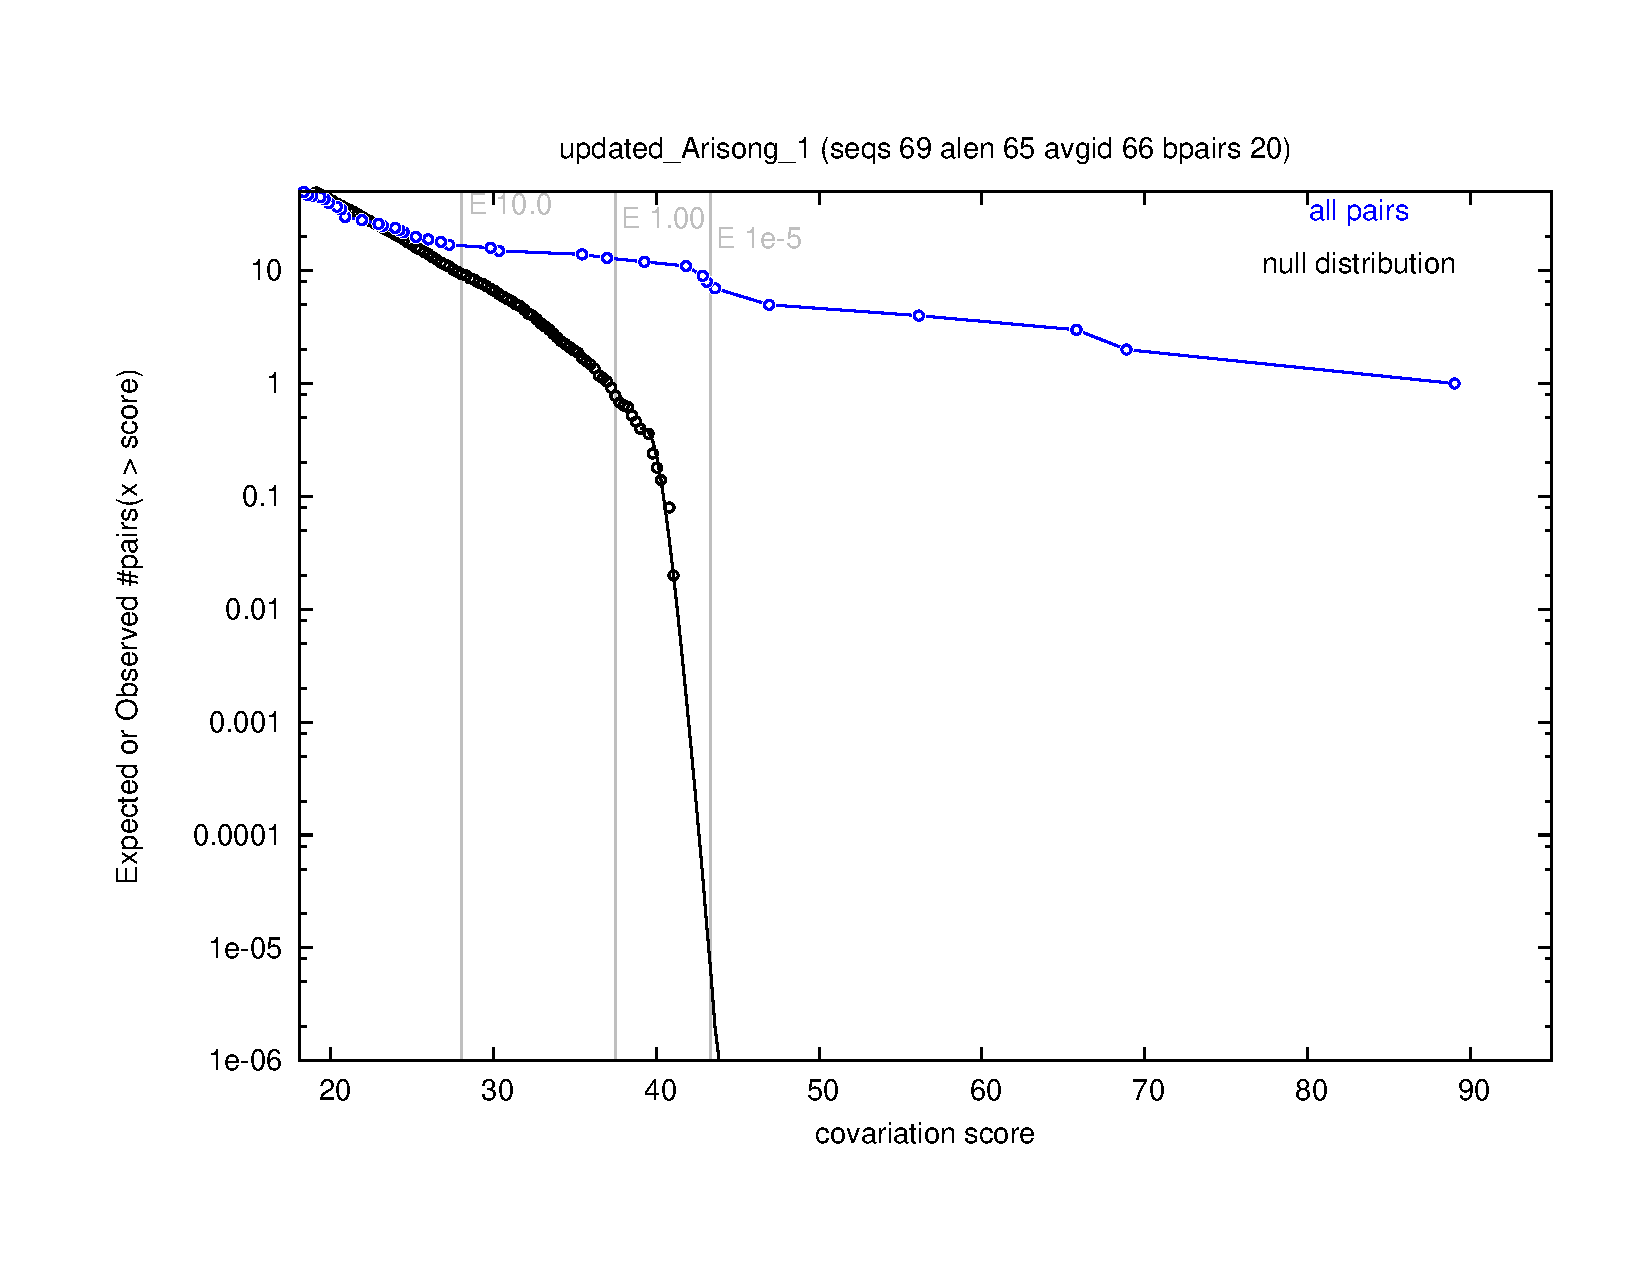
\includegraphics[scale=0.50]{Arisong_his.pdf} 
\caption{\small\textbf{\prog{tutorial/updated\_Arisong\_1.his.\{ps,svg\}}:
    covariation scores histogram.}  The histogram of scores for all
  pairs in the given alignment is depicted in blue. The histogram for
  the null alignments is depicted in black. A black line indicates to
  fit to a truncated Gamma distribution of the tail of the null
  distribution.}
\label{fig:histogram}
\end{figure}

\begin{figure}
  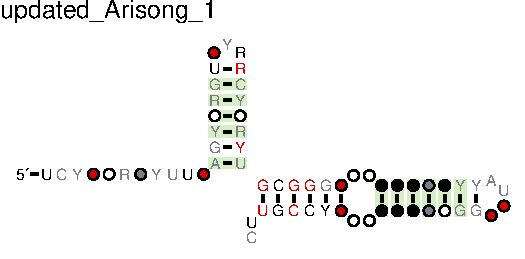
\includegraphics[scale=1.5]{Arisong_R2R.pdf} 
\caption{\small\textbf{\prog{tutorial/updated\_Arisong\_1.R2R.sto.\{pdf,svg\}}:
    annotated consensus secondary structure.} Base pairs with
  covariation scores equal or below the target E-value (0.05 as
  default) are depicted in green. By default only positions in the
  alignment with more than 50\% occupancy are depicted (unless they form
  a base pair). Option \prog{--r2rall} forces the depiction of all
  positions in the alignment.  }
\label{fig:r2r}
\end{figure}

\begin{figure}
  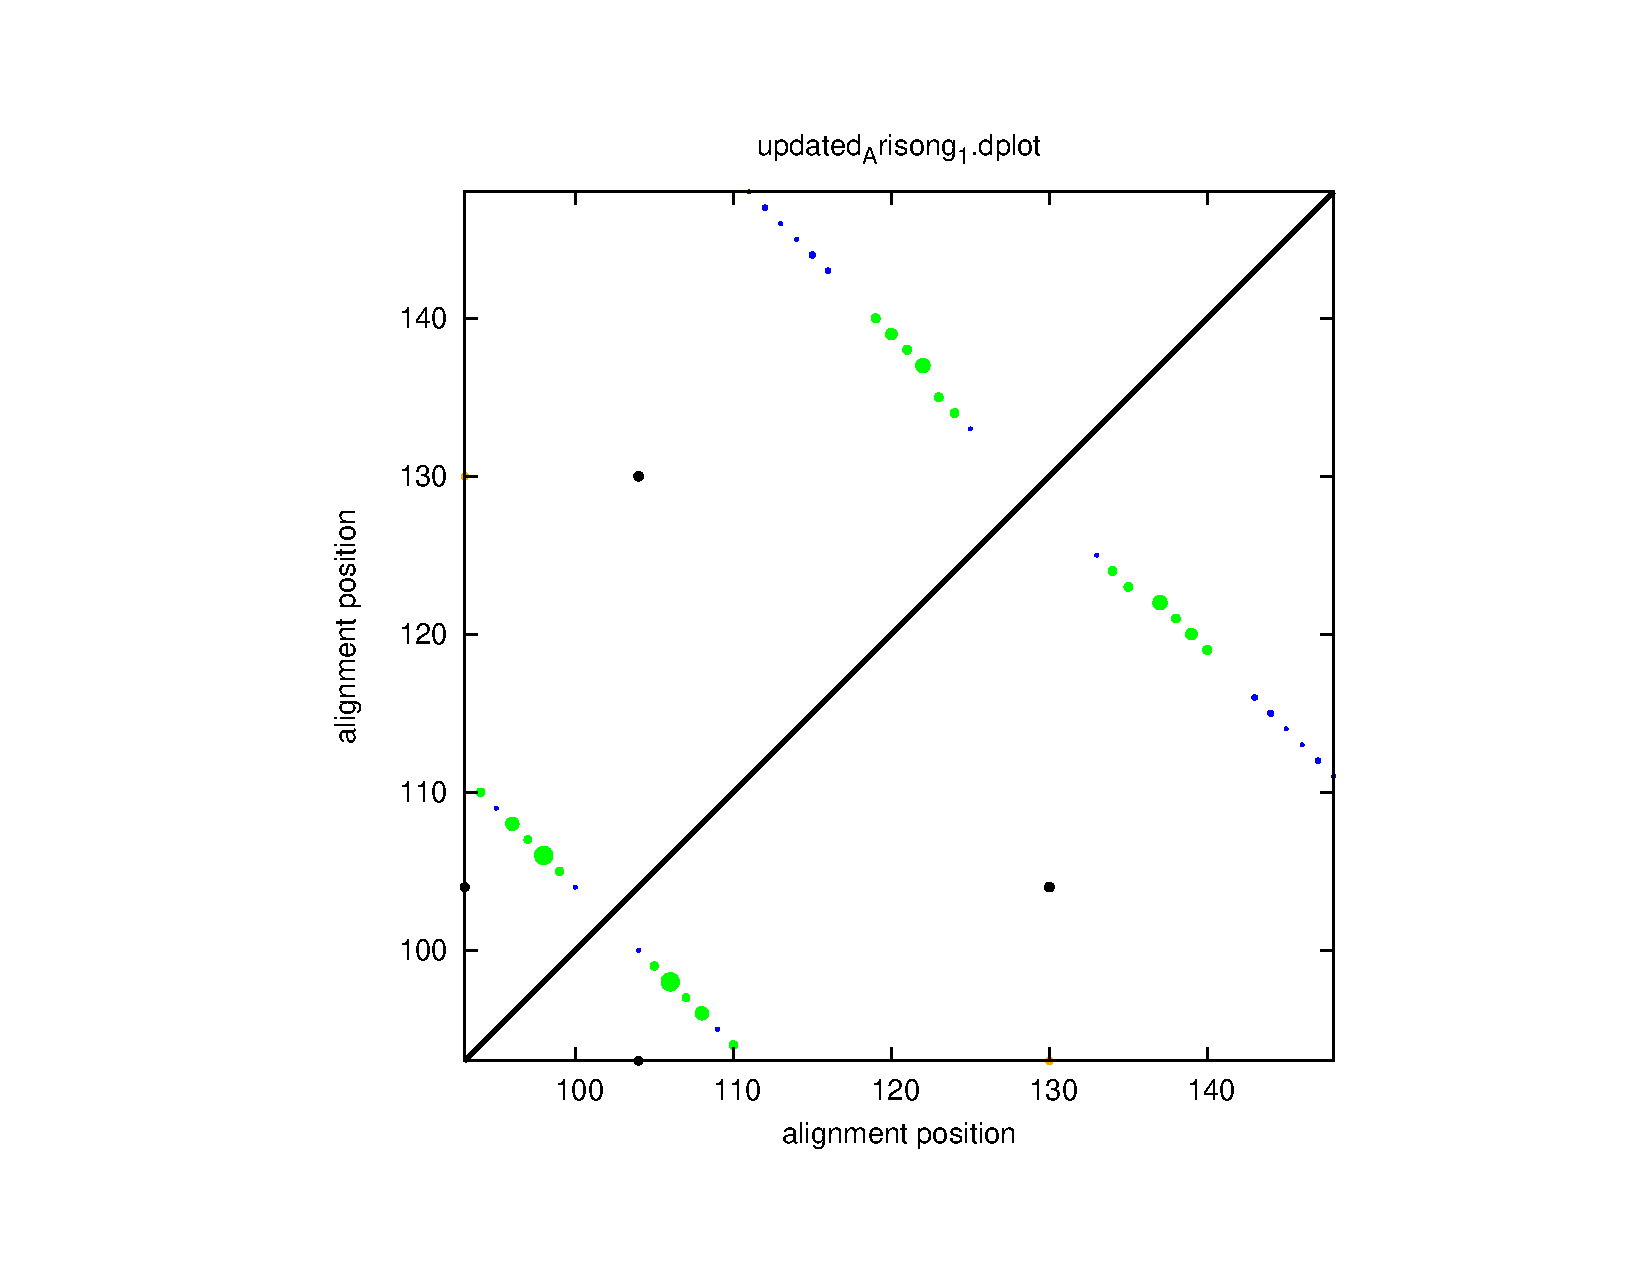
\includegraphics[scale=0.60]{Arisong_dplot.pdf}
\caption{\small\textbf{\prog{tutorial/updated\_Arisong\_1.dplot.\{ps,svg\}}:
    dotplot.}  Dot size is proportional to the covariation score. In
  blue we depict the consensus base pairs; in green, the consensus
  base pairs that show significant covariation; in orange other pairs
  that have significant covariation, are not part of the consensus
  secondary structure but are compatible with it; in black we depict
  other significant pairs.  Position are relative to the input alignment}
\label{fig:dplot}
\end{figure}



\clearpage
\subsection{Other tabular outputs}

\rscape\ produces two more tabular outputs per input file that are
more relevant for benchmarking purposes, such as:\\

File \prog{tutorial/updated\_Arisong.sum} looks lie:

\begin{sreoutput}
more tutorial/updated_Arisong.sum 
0.050000        updated_Arisong_1       69      65      65.16    GTp 9 20 20 45.000000 45.000000 
\end{sreoutput}


File \prog{tutorial/updated\_Arisong.roc} looks like:
\begin{sreoutput}
more tutorial/updated_Arisong.roc
# MSA nseq 69 alen 65 avgid 65.163163 nbpairs 20 (20)

# GTp thresh fp tf found true negatives sen ppv F evalue
89.04630 0 1 1 20 2060 5.00 100.00 9.52 0
88.79103 0 1 1 20 2060 5.00 100.00 9.52 0
88.53575 0 1 1 20 2060 5.00 100.00 9.52 0
88.28048 0 1 1 20 2060 5.00 100.00 9.52 0
88.02521 0 1 1 20 2060 5.00 100.00 9.52 0
87.76993 0 1 1 20 2060 5.00 100.00 9.52 0
87.51466 0 1 1 20 2060 5.00 100.00 9.52 0
...
\end{sreoutput}
